\subsection{Welcome Page}

\begin{center}
	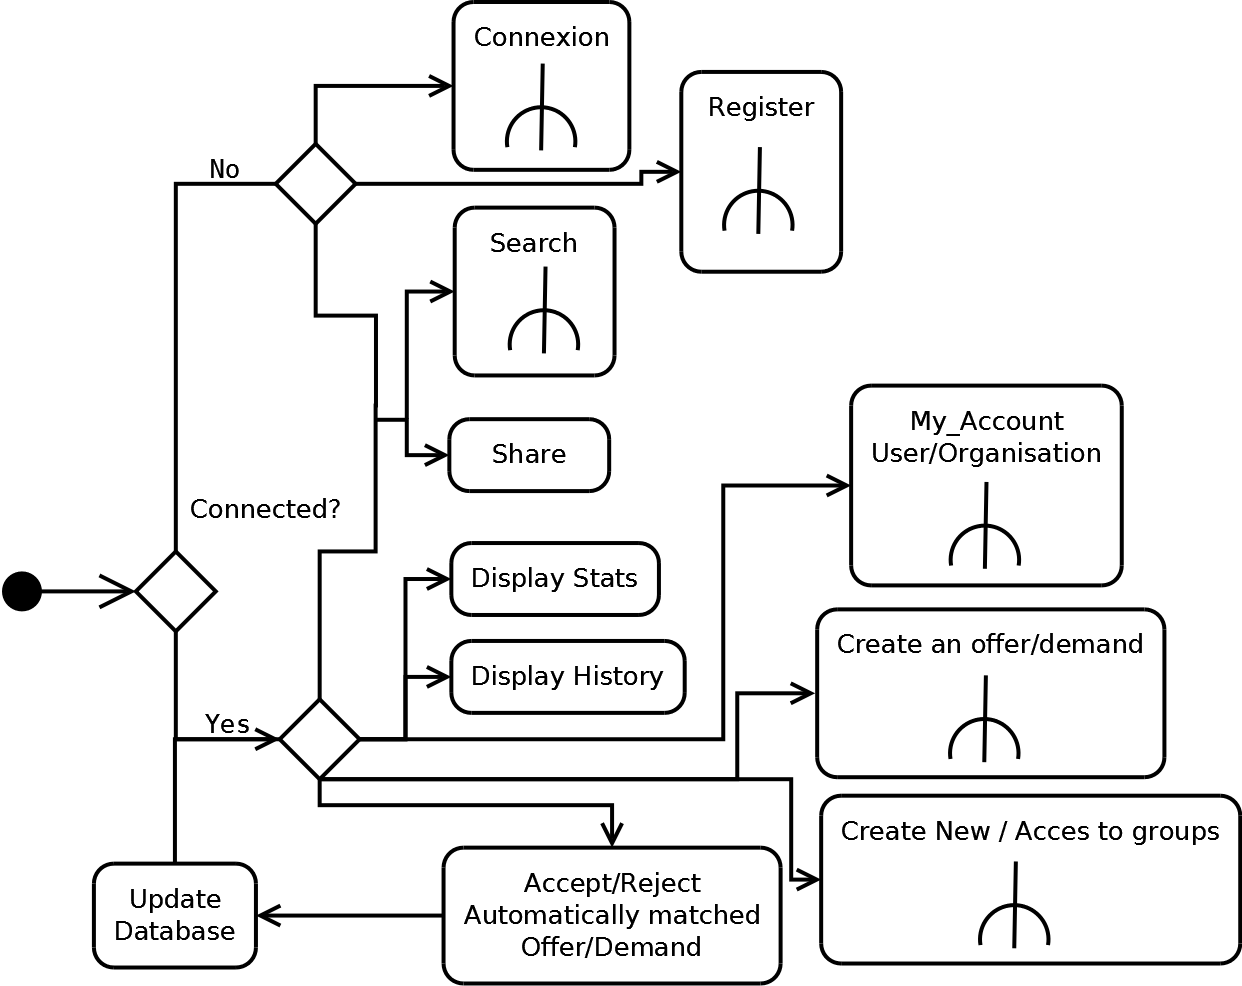
\includegraphics[width=.75\textwidth]{WelcomePage.png}
\end{center}
This diagram shows which functionalities are available to registered and unregistered users when they
connect to the welcome page. If the user is logged in, the website displays the different matching that have been made since his last visit so that the user can accept or reject those propositions.

\subsection{Connexion}

\begin{center}
	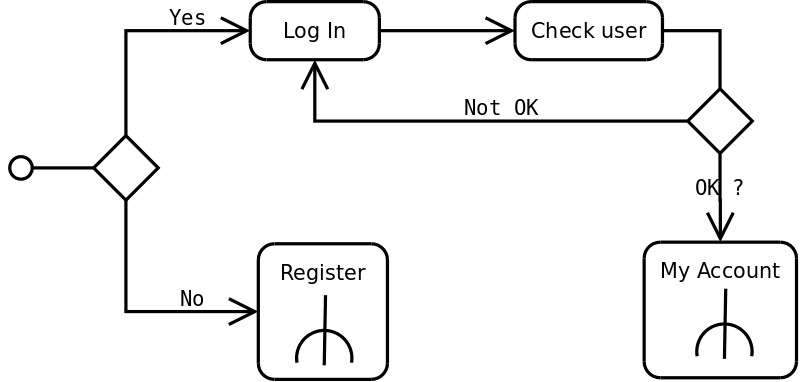
\includegraphics[width=.65\textwidth]{Connexion.png}
\end{center}
This diagram shows the interaction a user has with the website when he wants to be connected on the website.

\subsection{\texttt{MyAccount}: User}

\begin{center}
	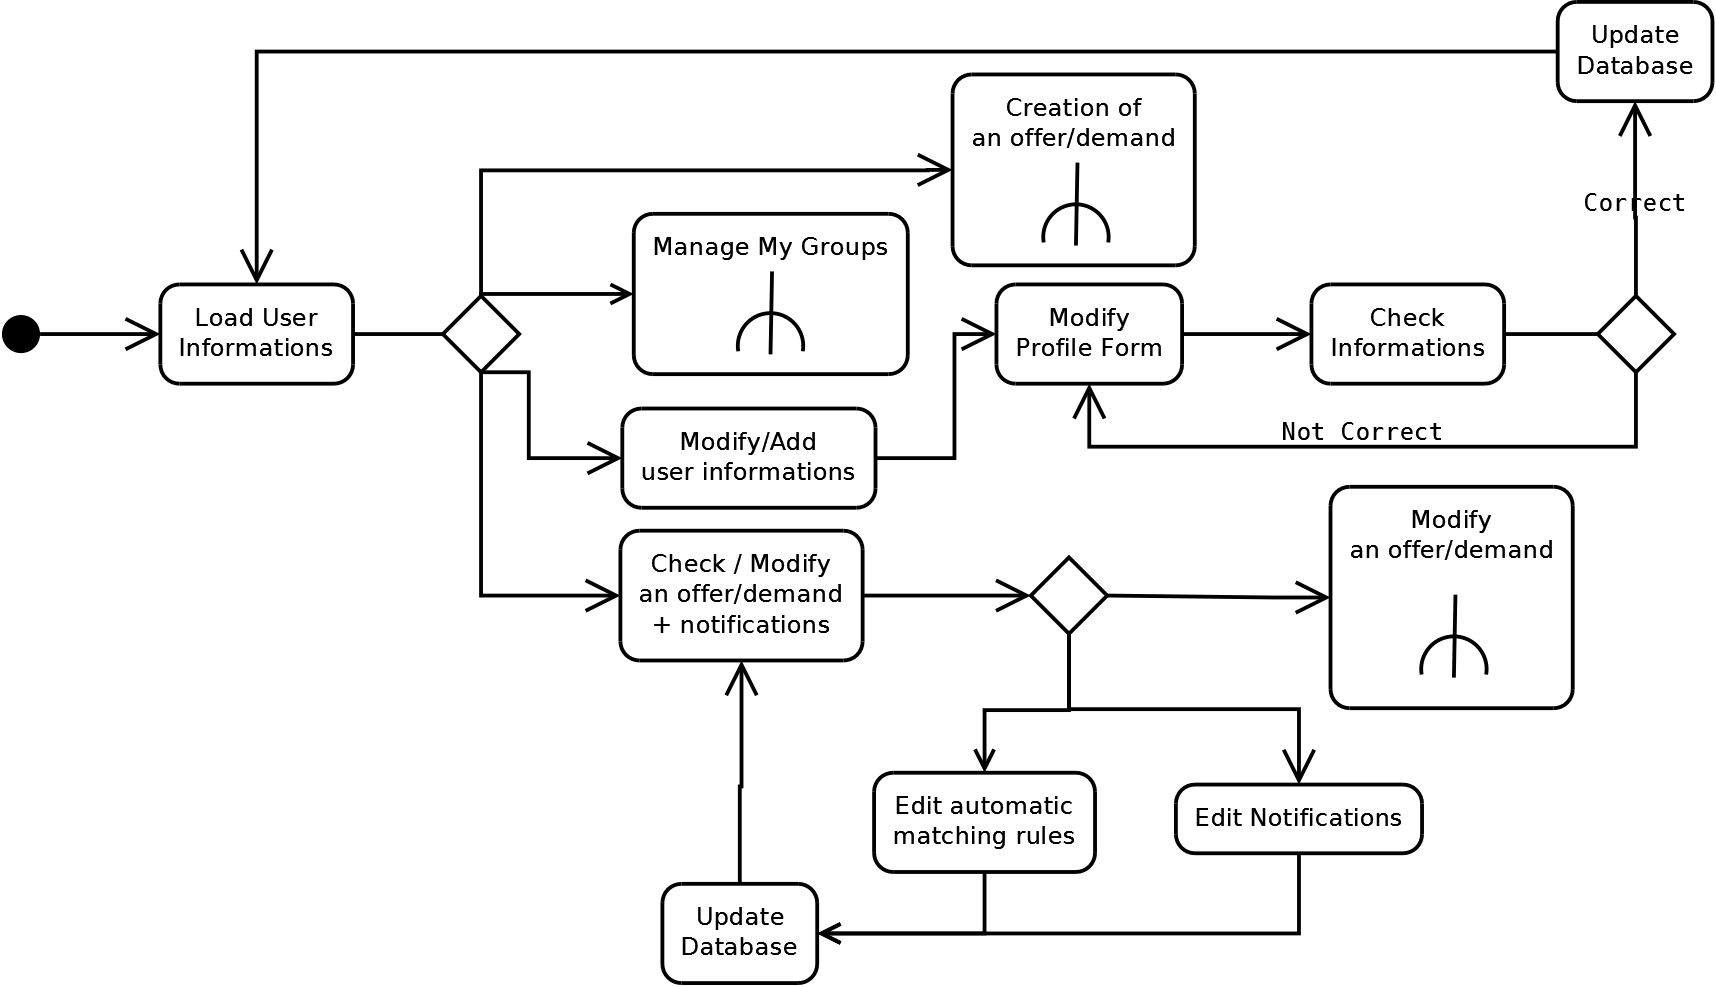
\includegraphics[width=1\textwidth]{MyAccount_User.png}
\end{center}
This diagram shows the possible interactions between a user and the website when he's on the main page after he log in. The user will be able to create a new offer/demand of services or to modify his profile informations. He can also manage offers/demands which he's subscribed to. The managing activity of groups is also made in this diagram.

\subsection{\texttt{MyAccount}: Organisation}

\begin{center}
	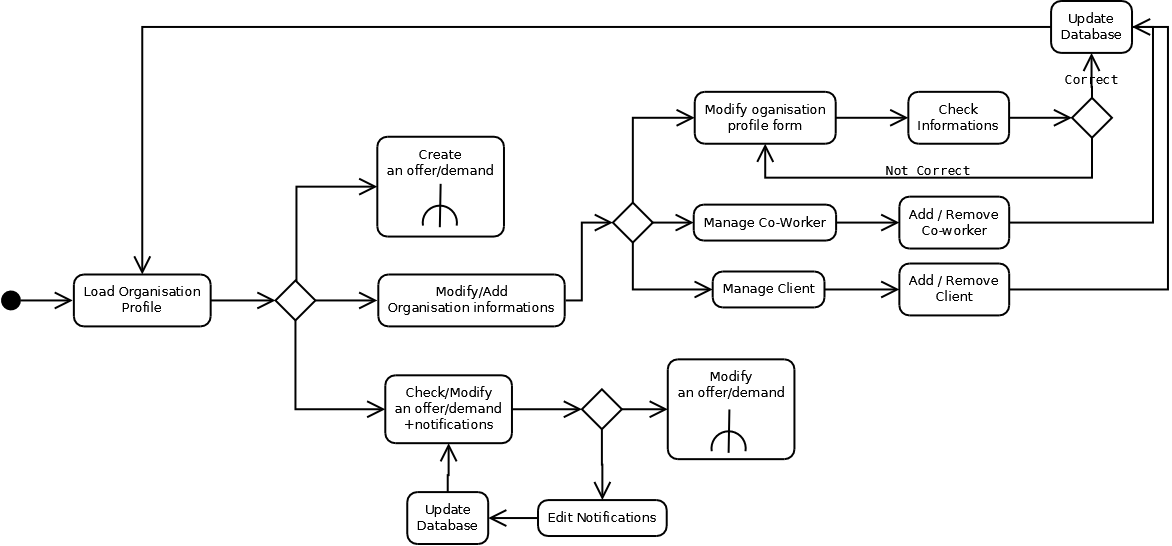
\includegraphics[width=1\textwidth]{MyAccount_Org.png}
\end{center}
Functionalities for organisations are basically the same as the ones for users. According to the requirements of the client, we will add functionalities to manage accounts of different clients (maybe people without any computer or internet connection at home), to create accounts for this clients and to manage a list of co-workers involved in the same organisation.

\subsection{Register}

\begin{center}
	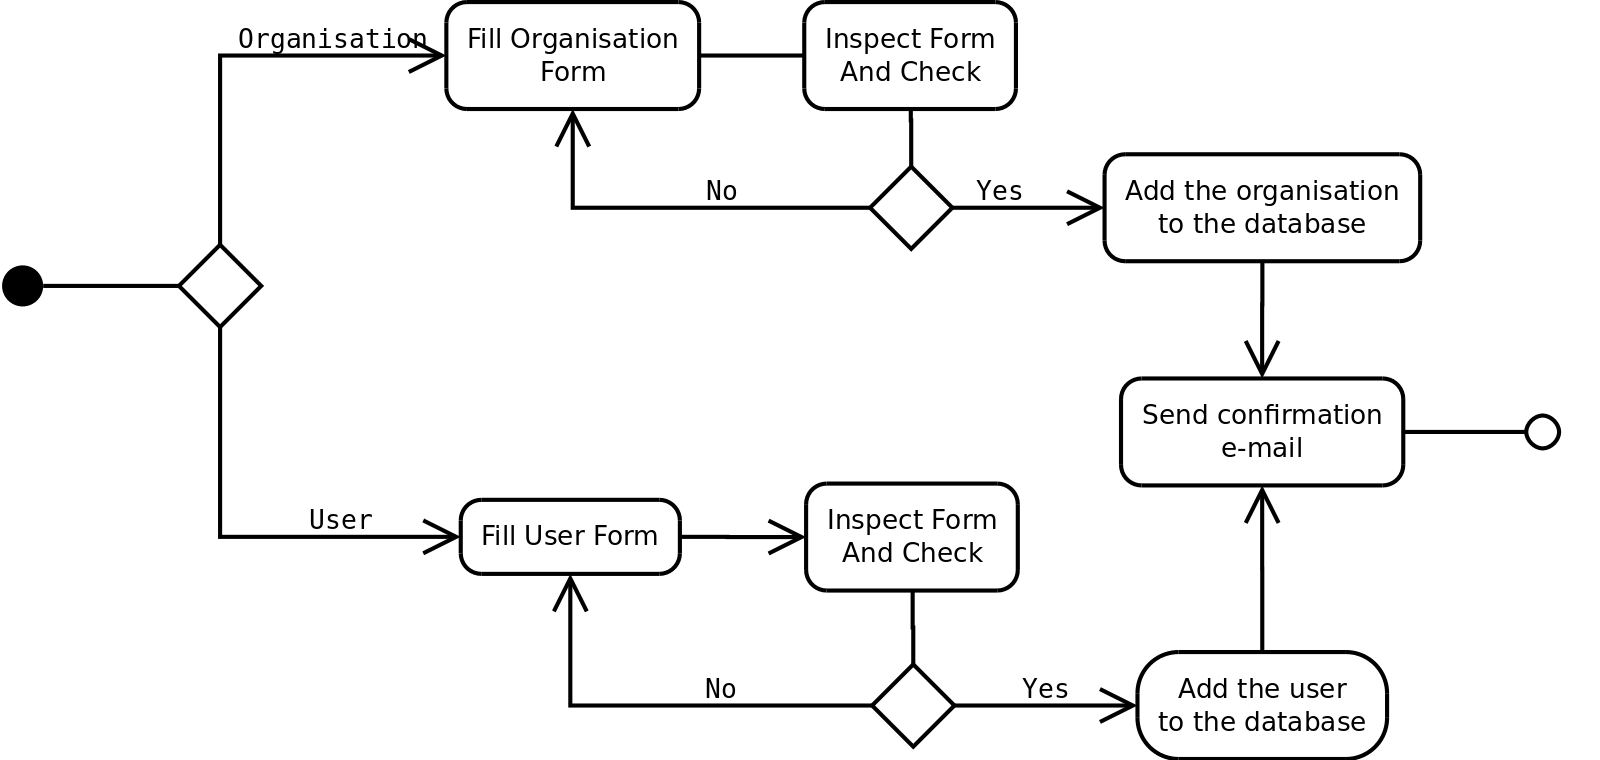
\includegraphics[width=.9\textwidth]{Register.png}
\end{center}
When a user wants to create an account, there are two possibilities:
\begin{itemize}
\item He can register as an organisation, there will be some checks to verify that it's a real social organisation. There will be a few more informations to give (like possible co-workers) into the form.
\item He can register as a user, either as a real user which need or provide service, or as a co-worker involved in an organisation. Co-workers profile are allowed only by an organisation.
\end{itemize}

\subsection{Group}

\begin{center}
	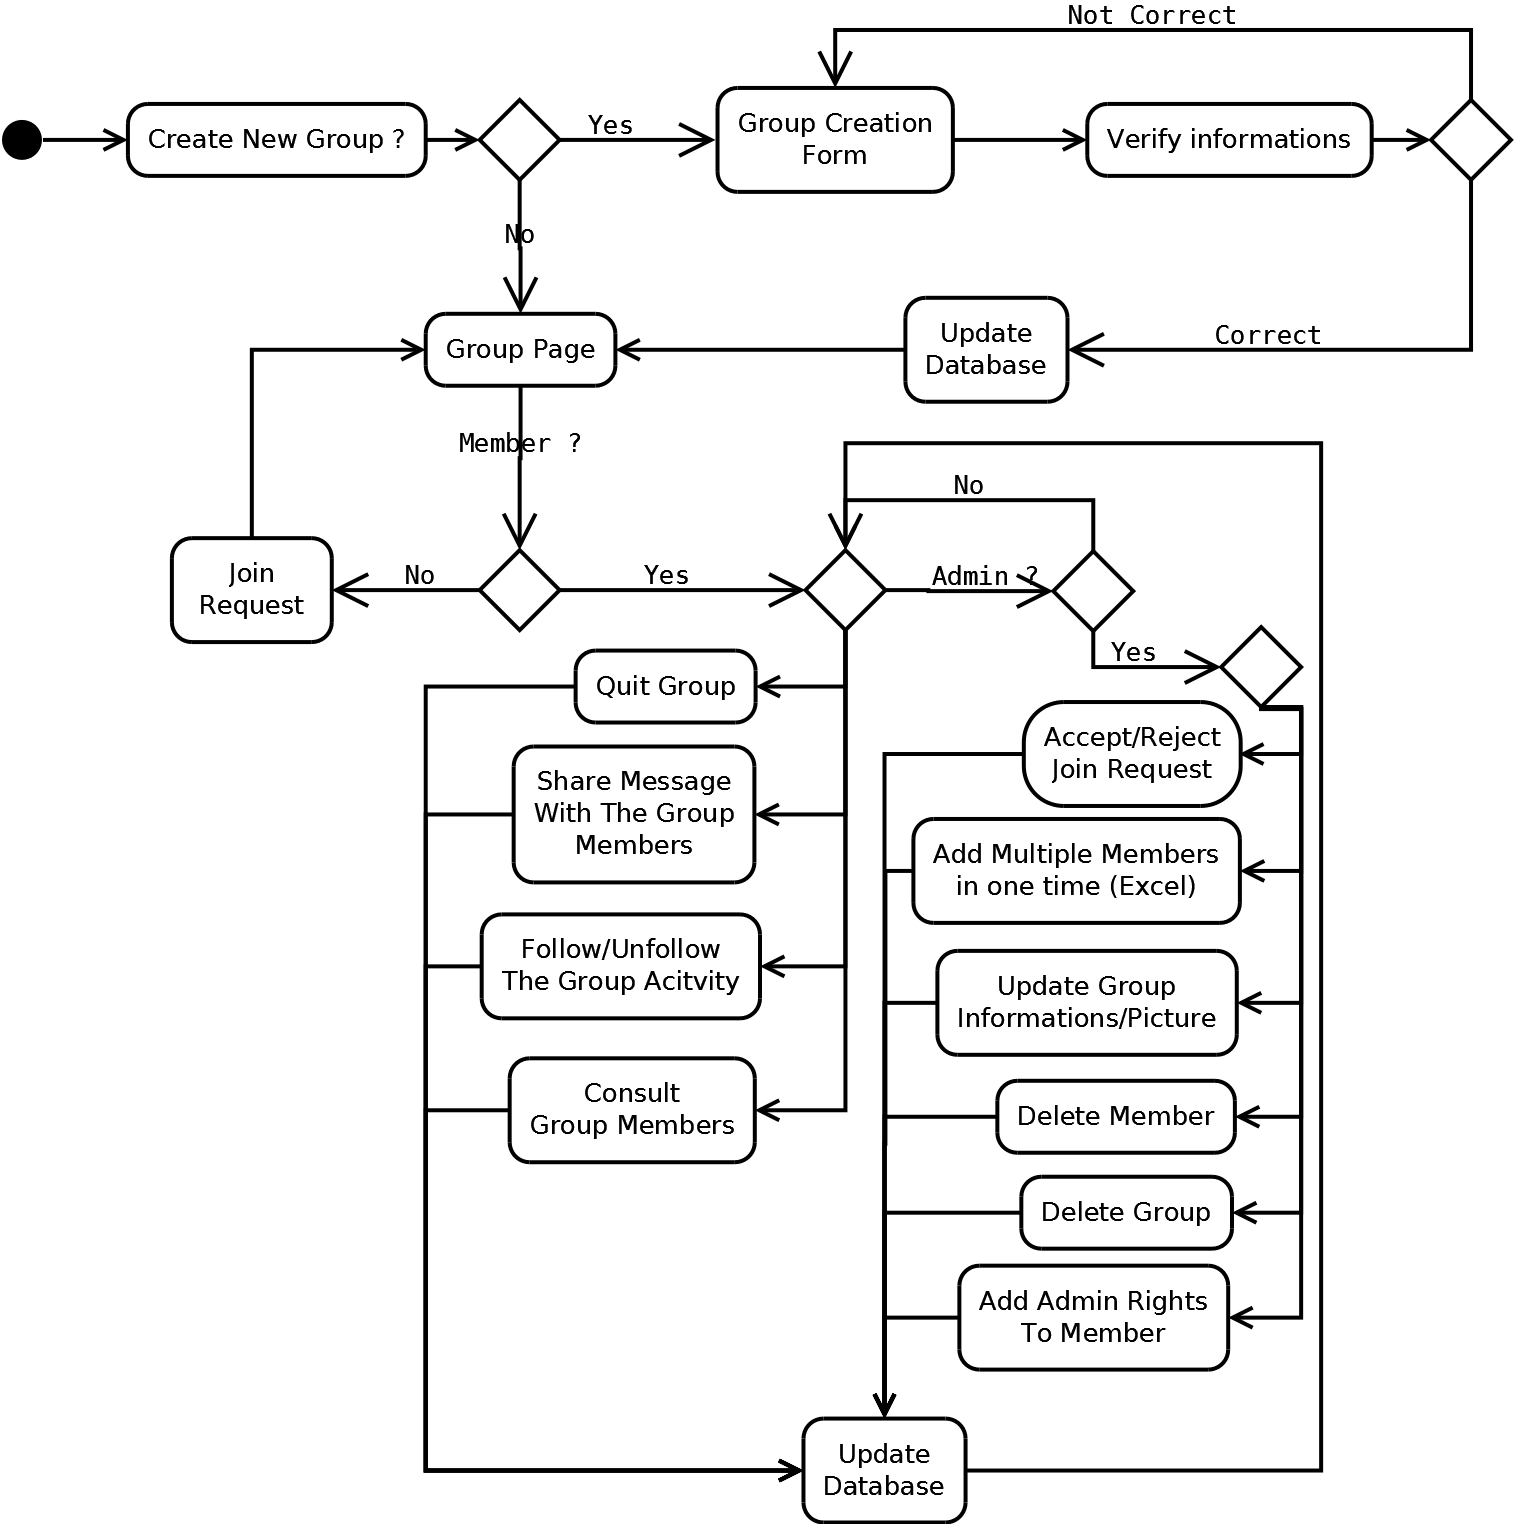
\includegraphics[width=.95\textwidth]{Group.png}
\end{center}
This diagram shows the different steps to create, manage and use a group, as an administrator and a (non) member of this group.

\subsection{Create or modify offers and demands}

\begin{center}
	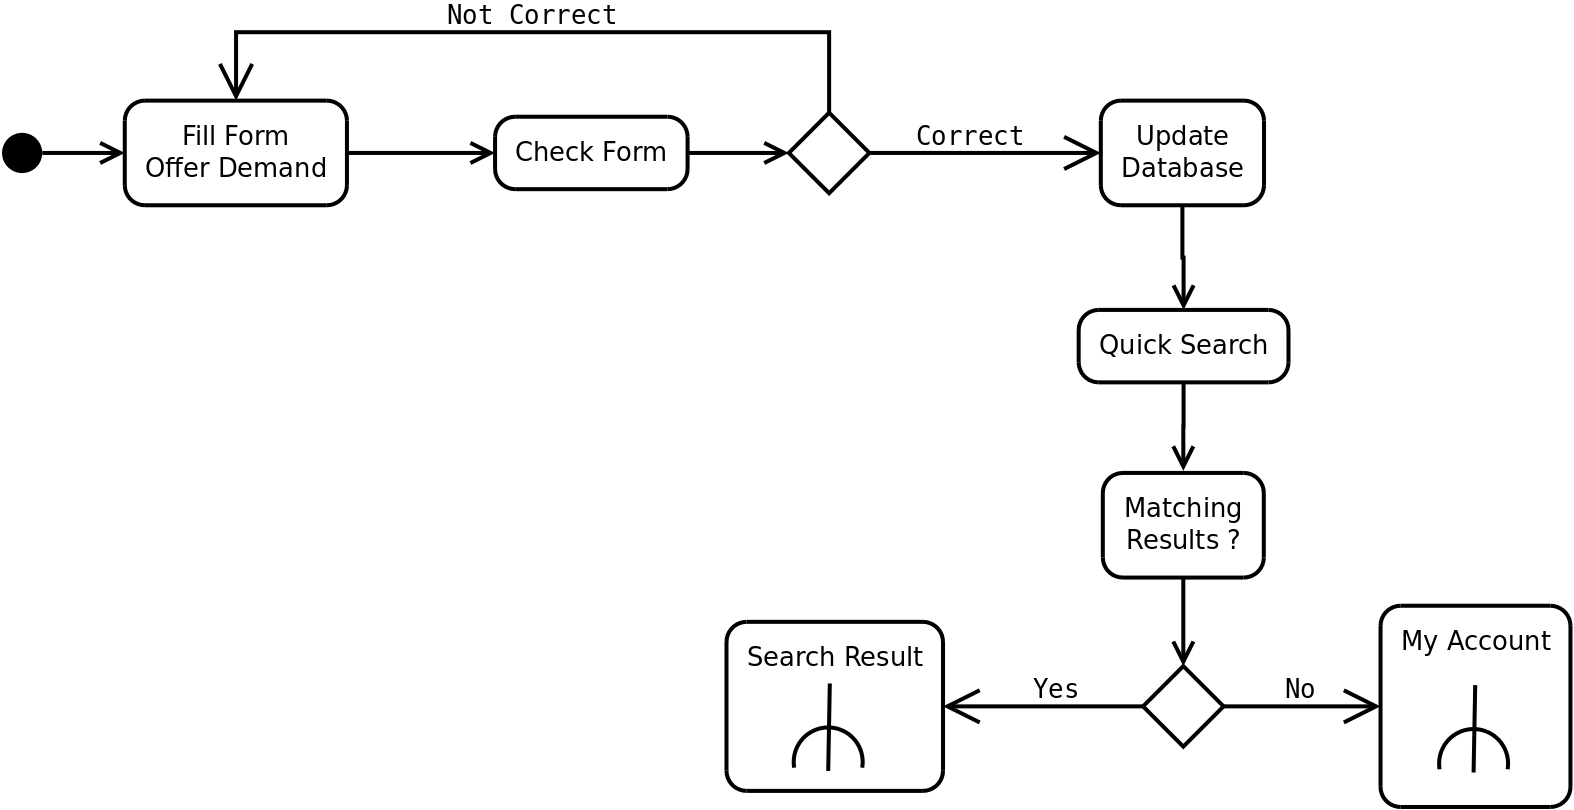
\includegraphics[width=.95\textwidth]{Create_Offer_Demand.png}
\end{center}
The user/organisation connected can at any moment create offers/demands of services. Organisation can create them for their clients. As soon as the offer/demand has been registered into the database, an immediate quick search is performed by the application. In case of successful search, results are automatically shown to the customer. Otherwise, the user is redirected to their account page.
As a standard user, you can also post a group offer/demand or an individual offer/demand.

\subsection{Search}

\begin{center}
	\hspace*{-1cm}
	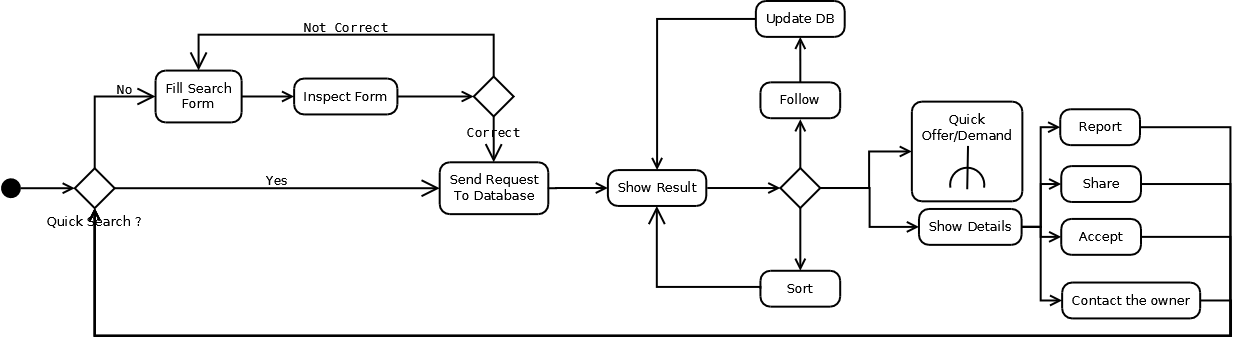
\includegraphics[width=1.1\textwidth]{Search.png}
\end{center}
There are two possible way to perform a search either on purpose (via the search button) or as the result of a matching while creating demand/offer. For each possible result, the customer can see the offer/demand's details individually, subscribe to one's he's interested in. If he wants to realise the service asked/offered, he can create a quick offer/demand which match the selected result. We assume that every demand as a corresponding offer and the opposite as well. 
